\documentclass[conference]{IEEEtran}
\IEEEoverridecommandlockouts
% The preceding line is only needed to identify funding in the first footnote. If that is unneeded, please comment it out.
\usepackage{cite}
\usepackage{amsmath,amssymb,amsfonts}
\usepackage{algorithmic}
\usepackage{graphicx}
\usepackage{textcomp}
\usepackage{xcolor}
\usepackage{balance}
% \usepackage{hyperref}
\usepackage[a-3u]{pdfx}
\def\BibTeX{{\rm B\kern-.05em{\sc i\kern-.025em b}\kern-.08em
    T\kern-.1667em\lower.7ex\hbox{E}\kern-.125emX}}
\begin{document}

\title{Capabilities2 for ROS2: Advanced Skill-Based Control for Human-Robot Interaction}

% \author{}
\author{
    \IEEEauthorblockN{Michael Pritchard, Kalana Ratnayake, Buddhi Gamage, Maleen Jayasuriya, Damith Herath}
    \IEEEauthorblockA{
    Collaborative Robotics Laboratory \\ 
    Faculty of Science and Technology \\
    University of Canberra \\
    \{Michael.Pritchard, Kalana.Ratnayakemudiyanselage,
    Buddhi.Gamage,
    Maleen.Jayasuriya,
    Damith.Herath\}@canberra.edu.au
    }
}
% \author{\IEEEauthorblockN{1\textsuperscript{st} Michael Pritchard}
% \IEEEauthorblockA{\textit{Faculty of Science and Technology} \\
% \textit{University of Canberra}\\
% Canberra, Australia \\
% michael.pritchard@canberra.edu.au}
% \and
% \IEEEauthorblockN{2\textsuperscript{nd} Kalana Rathnayake}
% \IEEEauthorblockA{\textit{Faculty of Science and Technology} \\
% \textit{University of Canberra}\\
% Canberra, Australia \\
% kalana.ratnayakemudiyanselage@canberra.edu.au}
% \and
% \IEEEauthorblockN{3\textsuperscript{rd} Buddhi Gamage}
% \IEEEauthorblockA{\textit{Faculty of Science and Technology} \\
% \textit{University of Canberra}\\
% Canberra, Australia \\
% buddhi.gamage@canberra.edu.au}
% \and
% \IEEEauthorblockN{4\textsuperscript{th} Maleen Surname}
% \IEEEauthorblockA{\textit{dept. name of organization (of Aff.)} \\
% \textit{name of organization (of Aff.)}\\
% City, Country \\
% maleen.jayasuriya@canberra.edu.au}
% \and
% \IEEEauthorblockN{5\textsuperscript{th} Damith Herath}
% \IEEEauthorblockA{\textit{dept. name of organization (of Aff.)} \\
% \textit{name of organization (of Aff.)}\\
% City, Country \\
% damith.herath@canberra.edu.au}
% }

\maketitle

\begin{abstract}
In the early days of the Open Source Robotics Foundation, a lesser-known project aimed to design an ''app-able robot'', leading to the creation of the ''Capabilities'' package for the Robot Operating System (ROS). Over a decade later, formulating robot capabilities remains a
significant technical hurdle in bringing robots from the lab into everyday life. This paper introduces \textit{Capabilities2}, a successor to the original Capabilities package, now reimagined for ROS2. Capabilities2 enhances the original design
by enabling advancements in skill-based control techniques and offering a more efficient, extensible framework for defining and utilising robot capabilities. We delve into its application in new real-world scenarios, with a particular focus on human-robot interactions
and the deployment of collaborative mobile robots in human-centric environments. Capabilities2 addresses challenges in implementing intuitive, collaborative robots by introducing an abstracted database handler, an object-relational mapping for
capability models, and a plugin architecture for capability execution. These features support dynamic capability representation, runtime adaptability, and integration with modern AI techniques for skill-based task planning. By providing a standardised yet flexible framework,
Capabilities2 reduces the integration effort required to develop top-level controls for real-world scenarios, facilitating rapid development and deployment. Our contributions include the reimplementation of the Capabilities package in ROS2, enhancements to support
contemporary robotic applications, and demonstrations of new use cases enabled by Capabilities2. We believe that Capabilities2 significantly advances the field of robotics by equipping developers with tools to create more capable, adaptable, and interactive robots. Capabilities2 is available at \url{https://github.com/CollaborativeRoboticsLab/capabilities2}
\end{abstract}

\begin{IEEEkeywords}
capability, interface, provider, communication, service, ROS2, API, package, skill, task, HRI
\end{IEEEkeywords}

\section{Introduction}
% Representations of skills, tasks, behaviours, and capabilities in robotics are numerous. Different approaches have been proposed that range from tightly defined instructive systems that are difficult to adapt, to broad and ambiguous models that leave room for adaptation but give rise to challenges in symbolism and grounding \cite{chen2024language,olivares2019review}. Skills, behaviours, and tasks are often part of the taxonomy of current state-of-the-art control problems solving the top-most level of a hierarchical control system \cite{mayr2023skiros2}; performing a task. Reference \cite{pantano2022capability} recently reviewed capability-based robot frameworks and described a divide between industrial representations emerging from industry 4.0, capability engineering, and academic robotics. Their review identified a prominent difference in complexity and effective parameterisation methods but concluded that most representations agree on a taxonomy based on task, skill, and primitive. They further concluded that there was weak standardisation leading to challenges in industry adoption. Most commonly in academia, modern representations are orchestrated using frameworks underpinned by behaviour trees (BT) \cite{colledanchise2021implementation} or hierarchical finite state machines (HFSM) \cite{ghzouli2023behavior}, with open source provisions including near-complete applications like FlexBe \cite{schillinger2016human}, SkiROS2 \cite{mayr2023skiros2}, and Knowrob \cite{tenorth2009knowrob}. To enable automated task planning using skills, these frameworks also implement knowledge representation with ontological standards like the resource description framework (RDF) \cite{mayr2023skiros2} and Web Ontology Language (OWL) \cite{van2004owl,pantano2022capability}. These ontologies relate to a world model that the system (often shared across multiple agents) must maintain \cite{rovida2017skiros}. Successful task planners have been demonstrated using symbolic AI \cite{olivares2019review}. A particular early ontology called ‘Capabilities’ was proposed by \cite{woodall2014ros}. This design leveraged the widely popular ROS middleware \cite{quigley2009ros} and presented an ontology that mapped ROS primitives to natural language descriptions of capabilities (or skills) using YAML. Relationships were limited to ‘dependency of’, ‘requires’, and ‘implemented by’. This approach was extremely simple and most prominently provided a generalised mechanism for creating robot user interface applications by way of implementing an abstraction used by different developers to interoperate. In contrast to more recent top-level control frameworks, the Capabilities package did not implement an explicit world model or formal ontology language. Recent developments in artificial intelligence research have yielded powerful alternatives to symbolic knowledge systems such as those used with RDF-based ontologies, with many proposing that hybrid approaches may be superior \cite{ahmad2023learning,chen2024language,mayr2022skill}. Techniques such as deep learning can learn patterns and relations directly without the need for designing rules. Further, they are capable of representing complex relationships continuously using vector spaces \cite{lecun2015deep}. As such, it is at this time relevant to consider how skill-based task planning may be achieved through connectionism and inference. The challenge with these approaches is providing suitable determinism and safety for industrial and commercial acceptance. These ideas become particularly relevant in robotics implemented for HRI since decent representations of skills, tasks, or behaviours become more difficult with a high degree of complexity, uncertainty, ambiguity, and heuristics. Further, skill taxonomies in HRI must be able to represent additional concepts such as role, level of interaction, proximity, and morphology \cite{yanco2004classifying}, which push the limit of most current skill-based ontological strategies. Therefore, the present paper argues that the Capabilities package (for ROS) is still relevant in the current robotics developer’s landscape. Summarily, developers need a way to share and reason about robot skills.  The tools should be simple, readily adaptable, and generalised. The framework should allow extension and specialisation and leverage the best technologies fit for purpose to evolve over time. The opensource ROS2 package can be found at: 

In human-robot interaction (HRI), representing and standardising robot skills, tasks, behaviours, and capabilities is crucial for effective collaboration and system adaptability. Various representations exist in robotics, ranging from rigid instructive systems that are difficult to adapt to flexible models that allow for adaptation but struggle with symbolism and grounding issues \cite{chen2024language, olivares2019review}. As robotics evolves, the need for a standardised framework for how robot skills are represented, executed, and integrated into systems becomes more apparent, especially in the context of industrial applications and HRI, where robots must perform tasks autonomously and in collaboration with humans.

Current state-of-the-art control systems often utilise hierarchical structures to manage tasks, skills, and behaviours \cite{mayr2023skiros2}. While industrial robotics have established frameworks based on Industry 4.0 principles, academic research remains diverse in its approaches. A recent review highlighted the divide between industrial and academic robotics, noting differences in complexity, parameterization, and the lack of standardisation \cite{pantano2022capability}. This fragmentation poses challenges for industry adoption, where consistent and reliable frameworks are needed.

In academia, robot skill representations are often orchestrated using symbolic approaches, where explicit knowledge is represented through predefined symbols and rules, allowing for clear task execution but limited adaptability. Commonly employed methods in this category include behaviour trees (BT) or hierarchical finite state machines (HFSM) which are widely adopted for organising and executing robot behaviours \cite{colledanchise2021implementation, ghzouli2023behavior}. Popular frameworks such as FlexBe \cite{schillinger2016human}, SkiROS2 \cite{mayr2023skiros2}, and Knowrob \cite{tenorth2009knowrob} incorporate these structures and extend their capabilities through knowledge representation standards like the resource description framework (RDF) \cite{mayr2023skiros2} and Web Ontology Language (OWL) \cite{van2004owl, pantano2022capability}. These ontologies effectively represent relations between skills, tasks, and system state, and enable systems to maintain a shared world model across agents, facilitating task planning and execution \cite{rovida2017skiros}. Early work on ontologies, such as the 'Capabilities' package for ROS \cite{woodall2014ros}, offered a simple but effective mechanism to map robot skills to natural language descriptions, enabling developers to create adaptable user interfaces.

However, recent advancements in artificial intelligence have led to the development of hybrid approaches that incorporate subsymbolic systems, such as deep learning-based models that can infer relationships and patterns without pre-defined rules \cite{ahmad2023learning, chen2024language, mayr2022skill}. These approaches, which operate in continuous vector spaces, show promise for skill-based task planning but face challenges in providing the determinism and safety required for industrial and commercial applications \cite{lecun2015deep}. This is particularly important in HRI, where the complexity of interactions, role differentiation, morphology, and spatial proximity introduce additional requirements for skill representation \cite{yanco2004classifying}.

Given these challenges, this paper introduces Capabilities2, an upgraded and re-implemented version of the original Capabilities package, reaffirming its continued relevance in the current robotics landscape. Capabilities2 offers a generalised, adaptable framework for representing skills, building relationships between them, and enabling flexible, skill-based intelligence within the ROS2 ecosystem. By enhancing the original design, it addresses previous limitations and introduces features such as an abstracted database handler, an object-relational mapping (ORM) for capability models, and a plugin architecture for capability execution.

We anticipate that the HRI community will benefit from this package, as it enables developers to reason about robot skills while offering flexibility for future developments. As HRI systems grow in complexity, Capabilities2 provides tools that are simple, extendable, and capable of integrating advanced technologies, which are essential for building robust and scalable robotic systems. Our contributions include the reimplementation of the Capabilities package in ROS2, enhancements to support contemporary robotic applications, and demonstrations of new use cases enabled by Capabilities2. By equipping developers with these tools, we aim to facilitate the creation of more capable, adaptable, and interactive robots.

\section{Design Goals}
In this endeavour, the present paper seeks to reimplement the ROS(1) Capability framework in ROS2 with the following aims:
\begin{itemize}
\item Introduce a suitable, adaptable standardisation framework for representing robot skills arising from ROS-based architectures.
\item Provide natural, rich, fluent, and descriptive representations of capabilities that sufficiently establish to entities outside the control system boundary ‘what this robot can do?’.
\item Provide an extensible API architecture that allows execution of a wide variety of robot skills, independent of the specific implementation.
\item Provide a reduction in integration effort required to produce top-level controls for real-world scenarios and specifically relevant to HRI environments to enable rapid development and deployment.
\item Enable common application security patterns for productionized ROS-based robots through password protection and access control arbitrated at the level of behaviours using a proxy such as Rosbridge \cite{crick2012ros}.
\end{itemize}

\section{The Capabilities(1) Package}

The Capabilities package implemented in ROS(1) provided a ROS service API to query and use capabilities. The capability knowledge was represented in interfaces that described the capability and the ROS primitives that were comprised, providers that defined specific implementations of an interface and details for using it, semantic interfaces that redefined interfaces using some semantic specificity, and remappings that contained a one-to-one mapping between a ROS primitive and a newly named ROS primitive. The design was implemented in Python using rospy \cite{quigley2009ros}. ROS Launch files were started and stopped at runtime by a capabilities server, meaning that the capabilities server was the only ROS primitive (node) that was required at start time. This provided resource management features to the end-user.

\section{The Capabilities2 Package}

\subsection{Expanding the Capabilities(1) Design}

Capabilities2 is designed to be more efficient and extensible. Major design components are implemented as C++ classes, APIs, or dynamically loaded classes (plugins) using the pluginlib\footnote{\url{https://github.com/ros/pluginlib}} library. This pattern of design follows other major ROS-based control frameworks such as Nav2 \cite{macenski2020marathon} and MoveIt2 \cite{coleman2014reducing} with a focus on performance, extensibility, abstraction, and low barrier to entry. Primary features present in Capabilities(1) are reimplemented using ROS primitives (primarily Services and Actions) and composition \cite{macenski2023impact}. Most notably, the design for launching capabilities via ‘roslaunch’ has been replaced. Instead, the execution of providers is abstracted using a plugin API called ‘runners’.

\begin{figure*}{
    \centering
    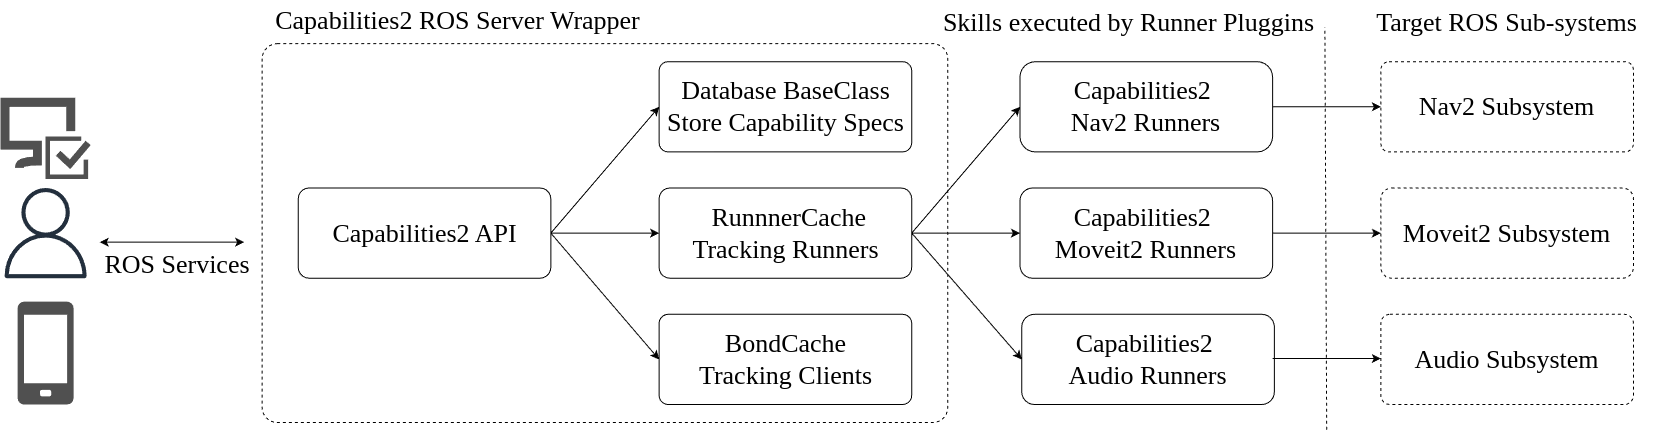
\includegraphics[width=0.9\linewidth]{figures/capabilities.drawio.png}
    \caption{The structure of the Capabilities2 Server (ROS Composable Node)}
    \label{fig:1}}
\end{figure*}

Capability models are implemented using an ORM and are stored in a database. This allows various features such as hot reloading, state persistence, and modularisable ontology. By embedding an abstracted database handler and ORM, Capabilities2 can be used to express more complex relationships between skills and tasks. In this way, capabilities can be used as a knowledge representation for a ROS2 network similar to other top-level control frameworks, while remaining adaptable to specialisation and new domains \cite{colledanchise2021implementation,mayr2023skiros2,tenorth2009knowrob}. A YAML-based data structure was retained as it provides arbitrary complexity of capability definition, allowing improvements to evolve over time and incrementally.
While an RDF database was not used in the initial implementation, the design provides an entry point for alternative databases and ORMs. 

An additional ROS service was implemented to allow registering capabilities at runtime. This allows skills to be added by spawners or service callers rather than using only YAML files exported through package manifests. This feature allows capabilities to be adapted during the operation of a robot through tuning or learning strategies. In conjunction with the database, these changes can be retained, a feature relevant to HRI to support individual differences. 

Comparison between Capabilities(1) and the Capabilities2 are mentioned in the Table \ref{table:1}.

\begin{table*}[]
\centering
\caption{Comparison of Capabilities1 and Capabilities2}
\label{table:1}
\begin{tabular}{lll}
\hline
\multicolumn{1}{c}{\textbf{Feature}} & \multicolumn{1}{c}{\textbf{Capabilities(1)}} & \multicolumn{1}{c}{\textbf{Capabilities2}} \\ 
\hline
\textbf{Architecture}                & Basic skill representation structure            & \begin{tabular}[c]{@{}l@{}}Modular design with plugin \\ support for flexibility and extensibility\end{tabular}                        \\
\hline
\textbf{Database Handling}           & In-memory only, fixed models                            & \begin{tabular}[c]{@{}l@{}}Abstracted database handler with\\ ORM support for better integration\end{tabular}                          \\
\hline
\textbf{Skill Representation}        & Symbolic-only representation                    & \begin{tabular}[c]{@{}l@{}}Dynamic capability representation with \\ AI integration for context-aware operations\end{tabular}          \\
\hline
\textbf{Runtime Adaptability}        & Static skill sets                               & \begin{tabular}[c]{@{}l@{}}Supports runtime adaptability, enabling real-time\\ changes through spawners and service calls\end{tabular} \\
\hline
\textbf{HRI Integration}             & General use cases                               & \begin{tabular}[c]{@{}l@{}}Tailored enhancements for HRI\\ applications for interactive systems\end{tabular}                    \\ 
\hline
\end{tabular}
\end{table*}

\subsection{New Capabilities Scenarios}

The major uses for Capabilities(1) proposed by \cite{woodall2014ros} comprised a user-friendly abstraction framework for multi-disciplinary development teams, improved system resource management through on-demand mechanisms, and a flexible development lifecycle through seamless simulation and real-world context switching. These features were achieved by using standardisation with capability interface models, capability use and free semantics, and contextual launch providers (launching different launch files). By implementing providers as plugins, capability execution can be more abstract, giving rise to new control mechanisms for capabilities above and beyond starting and stopping. For example, ROS actions and services can be used, and capabilities can be related and chained together. Further, BT actions or FSMs can be used. The major use cases that emerge from this design follow.

\begin{enumerate}
    \item \textbf{Simple interface for non-engineering HRI Researchers:}
    A person with limited prior experience working with robots can use Capabilities2 to obtain information such as ‘what can this robot do?’ and ‘how to use this robot?’ reducing the learning curve.
    \item \textbf{Portability of experiments between robots:}
    HRI experiments designed using Capabilities2 framework can be run on different robots without having to re-program from the scratch allowing for less experienced HRI researchers to work with robots.
    \item \textbf{Universal Mobile APP for robot control:}
    A Universal remote control application for robots could be created using Capabilities2 as standard interfaces. This will be useful for robot subsystem integrators to create robot apps, stores, or standardised sensors or actuators. This is made possible by the separation of capability specification and capability provider as proposed in capabilities(1) \cite{woodall2014ros}.
    \item \textbf{Bridging the communication gap between humans and robots:}
    HRI researchers can use generative AI to derive a task plan using capabilities as a knowledge base, and then request its execution via the runner API. This provides a connectionist implementation of automated task planning, circumventing some challenges using symbolic methods, whilst maintaining deterministic elements. Further, this is an extremely rapid approach to generating complex behaviours without the intervention of skilled programmers.
    \item \textbf{Improved robot and human security when in human-shared spaces:}
    By using an intermediate format for external interactions, more sensitive ROS primitives responsible for proper operation and safety do not need to be exposed. The capabilities server can be easily password protected. With a proposed implementation using a proxy is presented in Figure \ref{fig:2} \cite{crick2012ros}.   
\end{enumerate} 

\begin{figure*}{
    \centering
    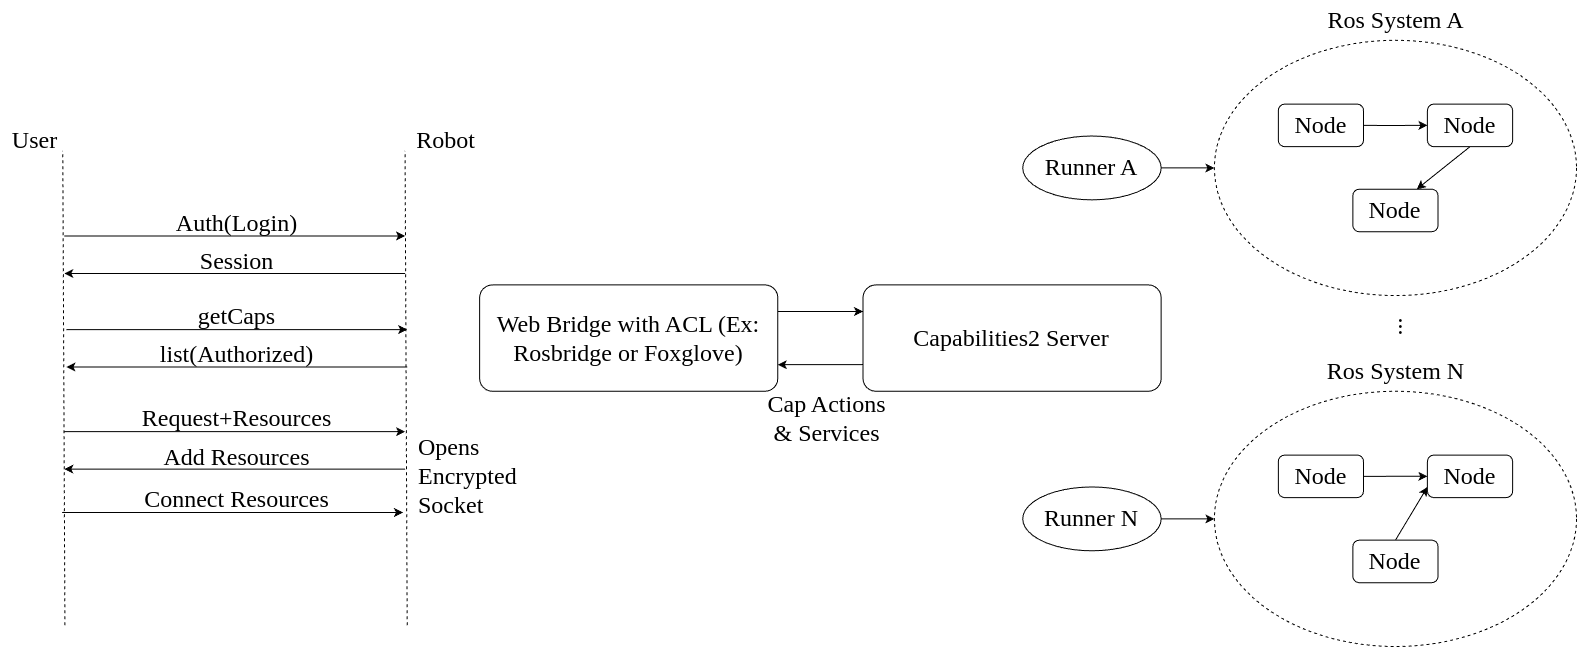
\includegraphics[width=0.9\linewidth]{figures/capabilities_authentication.drawio.png}
    \caption{An implementation of authentication/authorisation at the robot behaviour level using capabilities and a proxy \cite{alexander2012robot}. A proxy is used to provide authentication. A Capabilities server provides access control to subsystems at the skill or behaviour level. Subsystems are not directly accessed by external usage.}
    \label{fig:2}}
\end{figure*}

\subsection{A simple example using Capabilities2}

Suppose an HRI researcher needs to create a relatively expressive robot to undertake a user survey. In this scenario, the robot needs to ask a question and respond with different behaviours depending on the answer. A typical approach may be to explore off-the-shelf robots, then use a scripting tool to create each desired skill, and then put them together with implicit knowledge such as using if-else statements. While this approach works it poses challenges for reuse and replication, affecting the field as a whole. An alternative method is enabled with by Capabilities2.
First, the researcher finds suitable off-the-shelf Capabilities as designed by prior work. The researcher then models the desired behaviour in a formal ontology which may also form the basis of a more complex Capability. Then the researcher may publish the result and the methodology in an understandable, and reusable form, allowing others the reuse, reproduce, and compare. The added advantage of this approach is also a relative speed up in development and a shift in development focus to the task of most relevance the the present research.

\section{Discussion}

\subsection{Limitations}

To enable the launch functionality from capabilities(1) in capabilities2, a launch runner has been implemented. Due to the design of the launch system in ROS2\footnote{ \url{https://design.ros2.org/articles/roslaunch.html}}, it was necessary to create a launch proxy node that uses the Python3-based launch API to start and stop launch files. The launch runner uses an action to start, stop, and keep track of running launch files.

A world model was intentionally excluded to keep the package simple yet extensible. Implementing a turnkey world model poses domain-specific challenges, as different representations are suited to different problems \cite{davis2014representations}. In HRI, representations are often experimental or specialised and are closely tied to cognition, making them better suited for specialisation through plugins. Additionally, maintaining a world model within the capabilities system could cause inconsistencies by duplicating information provided by sub-systems (e.g., navigation maps). Instead, generating temporary world views queried by capabilities ensures a single source of truth derived from sub-systems.

\subsection{Future Work}

Capabilities2 is equivalent to Capabilities(1) in its features. It is extended to allow plugins. Future work will involve extending core features to enable HRI developers and researchers to rapidly implement high-level behaviours for further research and development and the sharing of tools. The areas that will be expanded include; implementing other database/ORM handlers including RDF and vector approaches. 

Reimplementing a `std\_capabilities' package to contain common skills, tasks, and primitives idiosyncratic to ROS robots. It was identified that closer design parity of the runner API with the behaviour tree framework would assist with composing multiple capabilities to perform complex tasks. Further, to support interaction with world models, a shared memory design for the runner API is in construction, supporting chaining runners together with a shared state. This will allow the development of an implicit world model and reactivity, with the advantage of only using that which is relevant and within the scope of the task (or runner) through a mechanism akin to views. The current design concept leverages the relatively popular lambda or functions-as-a-service methodology popularised in cloud computing.

\section{Conclusion}

The skill-based understanding of robots yields effective strategies for planning and executing complex tasks, as demonstrated through numerous implementations \cite{colledanchise2021implementation, mayr2023skiros2, pantano2022capability, woodall2014ros}. However, limitations exist when relying solely on symbolic planning, with hybrid machine learning strategies showing promise in overcoming these challenges \cite{yang2019program}.

% In this paper, we introduced the Capabilities2 package, which represents skills, provides a general framework for building relationships between them, and enables arbitrary skill-based intelligence on top of ROS2. By reimagining the original Capabilities package, Capabilities2 addresses the need for a standardized yet flexible framework that supports dynamic capability representation, runtime adaptability, and integration with modern AI techniques for skill-based task planning.

% This framework is especially relevant in highly multidisciplinary robotics domains such as HRI, as it supports interoperability and rapid integration through sensible and flexible standardization. Our contributions include the reimplementation of the Capabilities package in ROS2, enhancements to support contemporary robotic applications, and demonstrations of new use cases enabled by Capabilities2.

% We anticipate that the HRI community will benefit from this package, as it enables developers to reason about robot skills while offering flexibility for future developments. By reducing the integration effort required to develop top-level controls for real-world scenarios, Capabilities2 facilitates rapid development and deployment, ultimately bringing robots closer to everyday life.

In this paper, we introduced Capabilities2, a reimagined framework that represents skills, builds relationships between them, and supports skill-based intelligence on ROS2. By addressing dynamic capability representation, runtime adaptability, and AI integration, Capabilities2 provides a standardised yet flexible solution for modern robotics.

Particularly relevant in multidisciplinary domains like HRI, it facilitates interoperability and rapid integration, reducing the effort needed for top-level control development. By enabling efficient reasoning about robot skills and supporting future advancements, Capabilities2 accelerates deployment in real-world scenarios, advancing robots toward everyday applications.

\section{Acknowledgment}

Buddhi Gamage's and Kalana Ratnayake's research are supported by the University of Canberra Next-Gen Robotics – HRI Co-Funded Stipend Scholarship. 


\bibliographystyle{IEEEtran}
\balance
\bibliography{references}

\end{document}
